\documentclass{article}

\usepackage[french]{babel}
\usepackage[utf8]{inputenc}
\usepackage{listings}
\usepackage{graphicx}
\usepackage{float}
\usepackage{subcaption}
\usepackage{amsmath}
\usepackage{amssymb}
\usepackage{natbib}
\usepackage{hyperref}

\hypersetup{
    colorlinks=true,
    linkcolor=black,
    pdfborder={0 0 0} 
}

%%%%%%%%%%%%%%%% Lengths %%%%%%%%%%%%%%%%
\setlength{\textwidth}{15.5cm}
\setlength{\evensidemargin}{0.5cm}
\setlength{\oddsidemargin}{0.5cm}

%%%%%%%%%%%%%%%% Variables %%%%%%%%%%%%%%%%
\newcommand\projet{6}
\newcommand\titre{Résolution approchée d'équations différentielles / Modélisation de systèmes dynamiques}
\newcommand\groupe{3}
\newcommand\equipe{3}
\newcommand\responsible{Joao Pedro Neto De Abreu}
\newcommand\secretary{Pierre-Louis Shrestha--Salie }
\newcommand\others{Soufiane SBAI \\ Eve Turchet}

\begin{document}

%%%%%%%%%%%%%%%% Header %%%%%%%%%%%%%%%%
\noindent\begin{minipage}{0.98\textwidth}
  \vskip 0mm
  \noindent
  { \begin{tabular}{p{7.5cm}}
      {\bfseries \sffamily
        Projet \projet} \\ 
      {\itshape \titre}
    \end{tabular}}
  \hfill 
  \fbox{\begin{tabular}{l}
      {~\hfill \bfseries \sffamily Groupe \groupe\ - Equipe \equipe
        \hfill~} \\[2mm] 
      Responsable : \responsible \\
      Secrétaire : \secretary \\
      Codeurs : \others
    \end{tabular}}
  \vskip 4mm ~
\parbox{0.95\textwidth}{\small \textit{Résumé~:} \sffamily 
  Ce projet s'intéresse aux méthodes de résolution d'équations différentielles ainsi qu'à un certain nombre 
  d'applications possibles, notamment la modélisation de systèmes dynamiques. Nous étudierons la modélisation de 
  populations dite de Lotka-Volterra ainsi que la modélisation de système de réactions chimiques oscillantes.
  }
  \vskip 1mm ~
  

\end{minipage}

%%%%%%%%%%%%%%%% Main part %%%%%%%%%%%%%%%%

\tableofcontents

\newpage 

\section{Résolution d'équation différentielles}

Cette première partie traite de l'implémentation des méthodes numériques de résolution
d'équation différentielle.\\
Dans un premier temps, nous avons défini une répresentation des problèmes de Cauchy.\\
La solution initiale $y0$ est représentée par un array de float. La fonction différentielle est décrite
par une fonction Python $f(t, y)$ qui retourne un array de la même taille que $y$.

\subsection{Implémentation générique}

Nous avons implémenté quatre méthodes : Euler, Heun, point milieu et Runge Kutta.\\
Pour chaque méthode, on retrouve une fonction \texttt{step\_<name>(y, t, h, f)} qui effectue un seul pas de la méthode et 
une fonction \texttt{meth\_n\_step(y0, t0, N, h, f, step\_method)} qui applique la méthode sur N pas de taille constante.
Enfin, la fonction \texttt{meth\_epsilon(y0, t0, tf, eps, f, step\_method)} affine le pas jusqu’à atteindre une précision donnée.\\
Cette implémentation générique évite la duplication de code et facilite l'ajout d'une nouvelle méthode.


\subsection{Applications sur des équations différentielles connues}

Pour les quatres méthodes, la solution obtenue et la solution exacte sont extrêment proches pour la dimension 
une. Le tracé des résultats obtenus sont similaires pour les méthodes de Heun, du point milieu et de Runge
Kutta pour les dimensions une et deux. La figure~\ref{fig:heun} montre les résultats obtenus par la méthode de Heun.

\begin{figure}[ht]
    \centering
    \begin{subfigure}[b]{0.24\textwidth}
        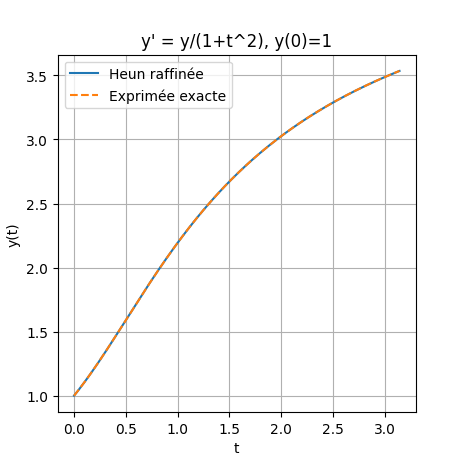
\includegraphics[width=\linewidth]{img/heun1.png}
    \end{subfigure}
    \hspace{0.01em}
    \begin{subfigure}[b]{0.49\textwidth}
        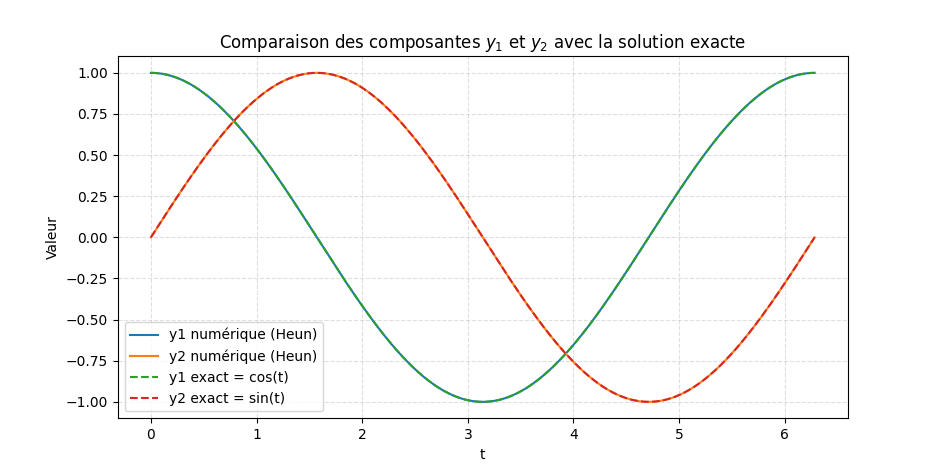
\includegraphics[width=\linewidth]{img/heun2.png}
    \end{subfigure}
    \hspace{0.01em}
        \begin{subfigure}[b]{0.24\textwidth}
        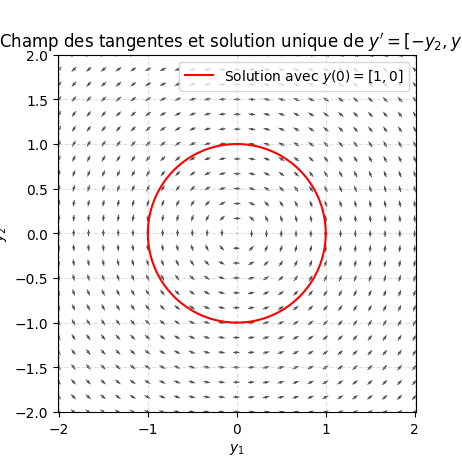
\includegraphics[width=\linewidth]{img/heun3.png}
    \end{subfigure}
    \caption{Résultats de la méthode de Heun}
    \label{fig:heun}
\end{figure}

Cependant, nous observons que la méthode d'Euler est moins précise
que les autres méthodes pour la dimension deux, comme le montre la figure~\ref{fig:euler}.

\begin{figure}[ht]
    \centering
    \begin{subfigure}[b]{0.24\textwidth}
        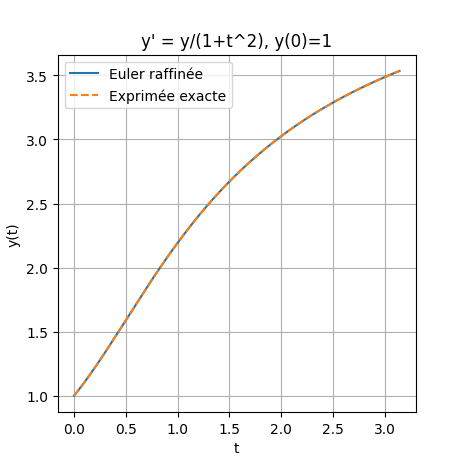
\includegraphics[width=\linewidth]{img/euler1.png}
    \end{subfigure}
    \hspace{0.01em}
    \begin{subfigure}[b]{0.49\textwidth}
        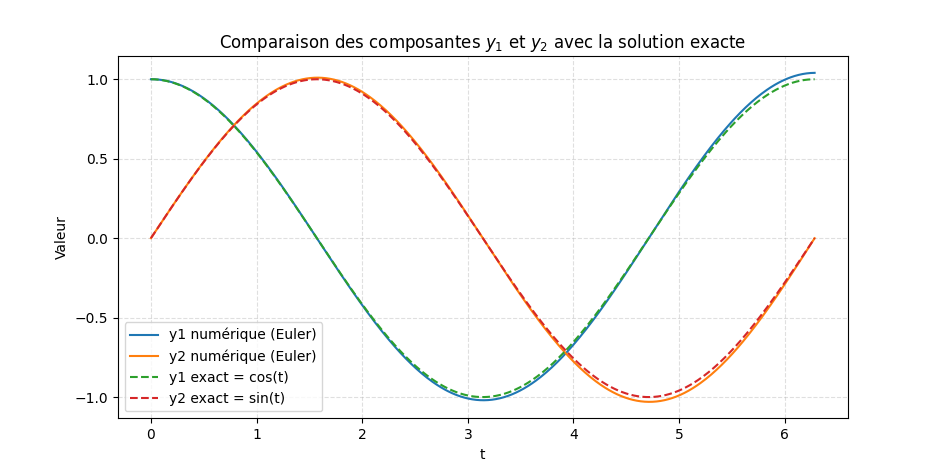
\includegraphics[width=\linewidth]{img/euler2.png}
    \end{subfigure}
    \hspace{0.01em}
        \begin{subfigure}[b]{0.24\textwidth}
        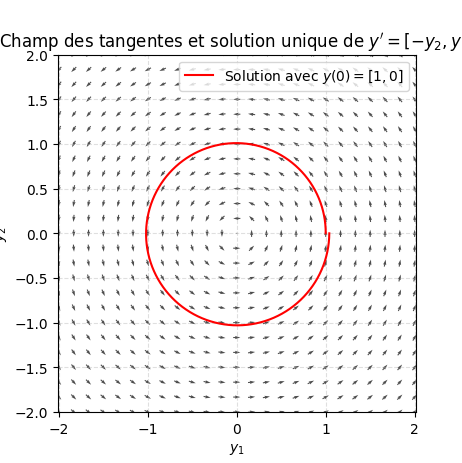
\includegraphics[width=\linewidth]{img/euler3.png}
    \end{subfigure}
    \caption{Résultats de la méthode d'Euler}
    \label{fig:euler}
\end{figure}

Les erreurs rencontrées sont en majorité des erreurs d'arrondis. En effet, l'approximation de la solution exacte par la 
méthode numérique introduit une erreur à chaque pas. De plus, pour des pas trop grand, la solution peut diverger.

\newpage 
\section{Modélisation de population}
Dans cette partie, nous allons nous intéresser à la modélisation de la population d'espèces.\\
Notre modélisation se base sur: les modèles malthusiens, le modèle de Verhulst ainsi que le système Proie-Prédateur décrit par Lotaka-Volterra.


\subsection{Modèles Malhusien et de Verhulst} 
Les modèles utilisés afin de décrire les variations d'une population sont les modèles malthusiens (\ref{eq:malthu}),ainsi que le modèle de Verhulst(\ref{eq:velhulst}).\\


%malthusiens
\begin{equation}
\frac{dN(t)}{dt} = bN(t) - dN(t) = \gamma N(t), \quad b, d > 0
\label{eq:malthu}
\end{equation}

%velhulst
\begin{equation}
\frac{dN(t)}{dt} = \gamma N(t) \left(1 - \frac{N(t)}{\kappa} \right), \quad \gamma, \kappa > 0 
\label{eq:velhulst}
\end{equation}


Avec :
\begin{enumerate}
\item $N(t)$, la fonction décrivant la variation de population
\item  $b$, le taux de reproduction de la population
\item $d$, le taux de décès de la population
\item $\gamma$,le taux de croissance de la population 
\item $\kappa$, la capacité maximale de la population
\end{enumerate}


\[
\frac{dN(t)}{dt} = \text{naissances} - \text{morts}
\]

Ces modèles décrivent notamment les variations de population à l'aide d'équations différentielles.
Les équations différentielles permettent de modéliser l'évolution d'une population car elles décrivent les variations du nombre d'individus en fonction du temps, en tenant compte des mécanismes de naissance et de mortalité.

\subsubsection{Résolution des équations différentielles}
Nous allons résoudre les modèles décrits précédemment numériquement à l'aide de Runge-Kutta pour des paramètres : $\gamma = 0.3, \kappa = 150$ et une population de départ de 100 individus sur un intervalle de temps d'une unité de temps.\\
À la fin du temps d'étude, les populations sont d'environ 2008 pour le modèle Malthusien, contre 146 pour le modèle de Verhulst.
\\
Pour les mêmes paramètres à l'exception d'une croissance $\gamma = -0.3$ : la population décrite par le modèle Malthusien est de 5 individus, contre 7 pour Verhulst.
% \textbf{Malhusien : } 
%
% \textbf{Verhulst:}
% \[
% \frac{dN}{dt} = \gamma N \Rightarrow N(t) = N_0 e^{\gamma t}
% \]
% \[
% \frac{dN}{dt} = \gamma N \left(1 - \frac{N}{\kappa} \right) 
% \Rightarrow 
% N(t) = \frac{\kappa}{1 + \left( \frac{\kappa - N_0}{N_0} \right) e^{-\gamma t}}
% \]
%

On remarque que le modèle malthusien est à croissance exponentielle. Ce caractère limite la portée du modèle, notamment pour l'étude de populations dans un environnement limité en ressources.
Le modèle de Verhulst offre une croissance sigmoïdale, qui va tendre vers $\kappa$. Cette stabilisation, à l'inverse du modèle Malthusien, semble plus réaliste dans ce cas d'environnement à ressources limitées.

\subsection{Modèle Lotka-Volterra}
Afin d'étudier l'évolution de plusieurs populations, nous allons nous intéresser au modèle \textbf{Lotka-Volterra}\ref{eq:lotka_volterra}.
\begin{equation}
\begin{cases}
\displaystyle \frac{dN(t)}{dt} = N(t)\big(a - bP(t)\big) \\
\displaystyle \frac{dP(t)}{dt} = P(t)\big(cN(t) - d\big)
\end{cases}
\quad \text{où } a, b, c, d > 0
\label{eq:lotka_volterra}
\end{equation}
Cette équation peut modéliser les interactions entre deux populations : les proies (notées $N$) et les prédateurs (notés $P$) car les taux de mortalité de la population proie sont liés au nombre de prédateurs présents dans l'environnement.
De même, pour les prédateurs, leur taux de natalité est conditionné par le nombre de proies disponibles.\\

En utilisant la méthode de Runge-Kutta, nous pouvons simuler les populations au travers du temps : (Figure \ref{fig:lotka})
\begin{figure}[h]
    \centering
    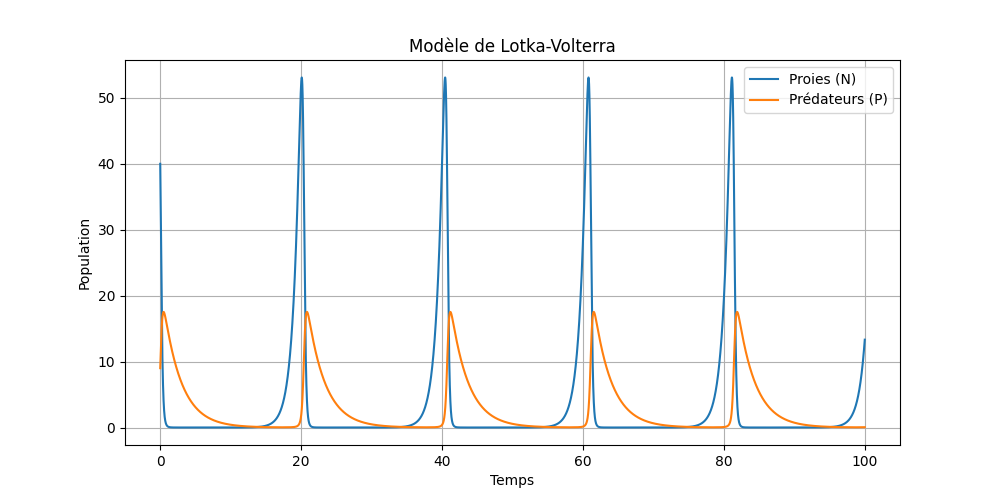
\includegraphics[width=0.4\textwidth]{img/ltka_volterra.png}
    \caption{Evoluions des populations proie et prédateur}
    \label{fig:lotka}
\end{figure}

Nous remarquons que les variations des populations oscillent de manière régulière. En traçant les variations du couple $(N(t), P(t))$ (Figure \ref{fig:phase}), nous observons des solutions périodiques. Les solutions constantes sont les points tels que $N = 0, P = 0$.
\begin{figure}[h]
    \centering
    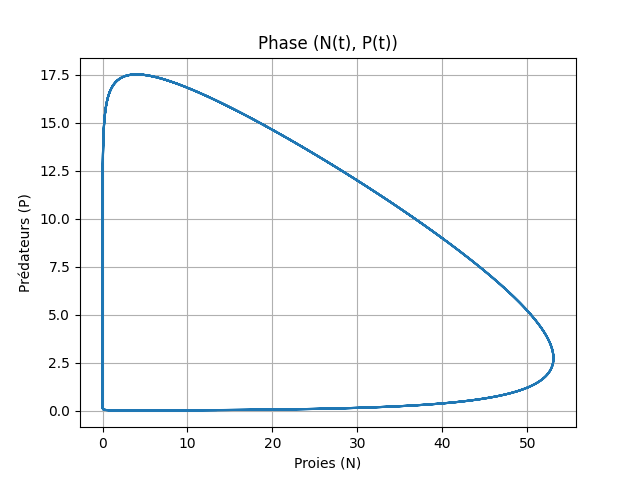
\includegraphics[width=0.4\textwidth]{img/phase.png}
    \caption{Variations du couple $(N(t), P(t))$}
    \label{fig:phase}
\end{figure}
Nous pouvons calculer cette période à l'aide du module \textit{scipy} de Python. Dans l'exemple décrit précédemment, la période est d'environ 20.35.
\subsubsection{Solutions proches du point $y_0$}
Pour un point $y_0$, nous pouvons calculer les variations entre les solutions partant de conditions initiales proches.
Comme présenté sur la figure \ref{fig:local_y0} pour le point initial $(1, 1)$. On remarque que les solutions forment un cercle autour du point.
Nous remarquons également que la forme du diagramme dépend du point initial. 
\begin{figure}[h]
    \centering
    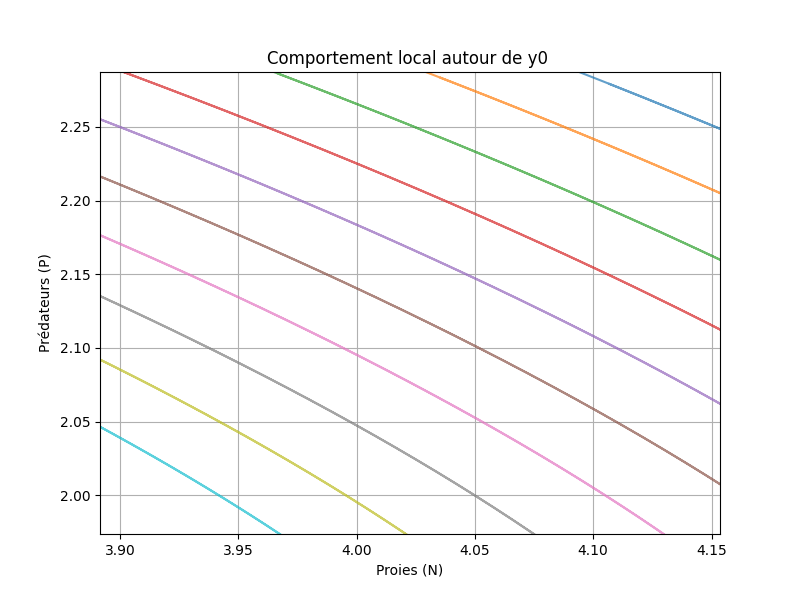
\includegraphics[width=0.4\textwidth]{img/local_y0.png}
    \caption{Variations du couple $(N(t), P(t))$}
    \label{fig:local_y0}
\end{figure}
\subsubsection{Points singuliers}
Nous pouvons calculer des solutions constantes en étudiant les valeurs de $t$ telles que $\frac{dN(t)}{dt} = 0, \frac{dP(t)}{dt} = 0$.\\
On trouve des solutions constantes lorsque $N = 0, P = 0$, également lorsque $N = \frac{d}{c}, P = \frac{a}{b}$.
Nous remarquons que les solutions autour d'un point singulier forment une série autour du point.



\cite{TODOREMOVEJKj}

\section{Réactions chimiques oscillantes}

Nous étudions ici des réactions chimiques oscillantes, notamment la réaction de Belousov-Zhabotinsky, à travers un modèle simplifié à trois dimensions :

\begin{equation}
    \begin{aligned}
        \frac{dX}{dt} &= 10 + bZ - X - XY^2\ \text{, }
        \frac{dY}{dt} &= 200(X + XY^2 - Y) \ \text{, }
        \frac{dZ}{dt} &= 50(Y - Z) \
    \end{aligned}
\end{equation}

Avec des conditions initiales fixées à $[1; 0; 0]$, nous étudions l'évolution du système en fonction du paramètre $b$.

\subsection{Résolution numérique et premiers résultats}

Le système est résolu numériquement à l'aide de la méthode de Runge-Kutta d'ordre 4. La figure suivante montre l'évolution de $Y(t)$ pour différentes valeurs de $b$ :

\begin{figure}[H]
\centering
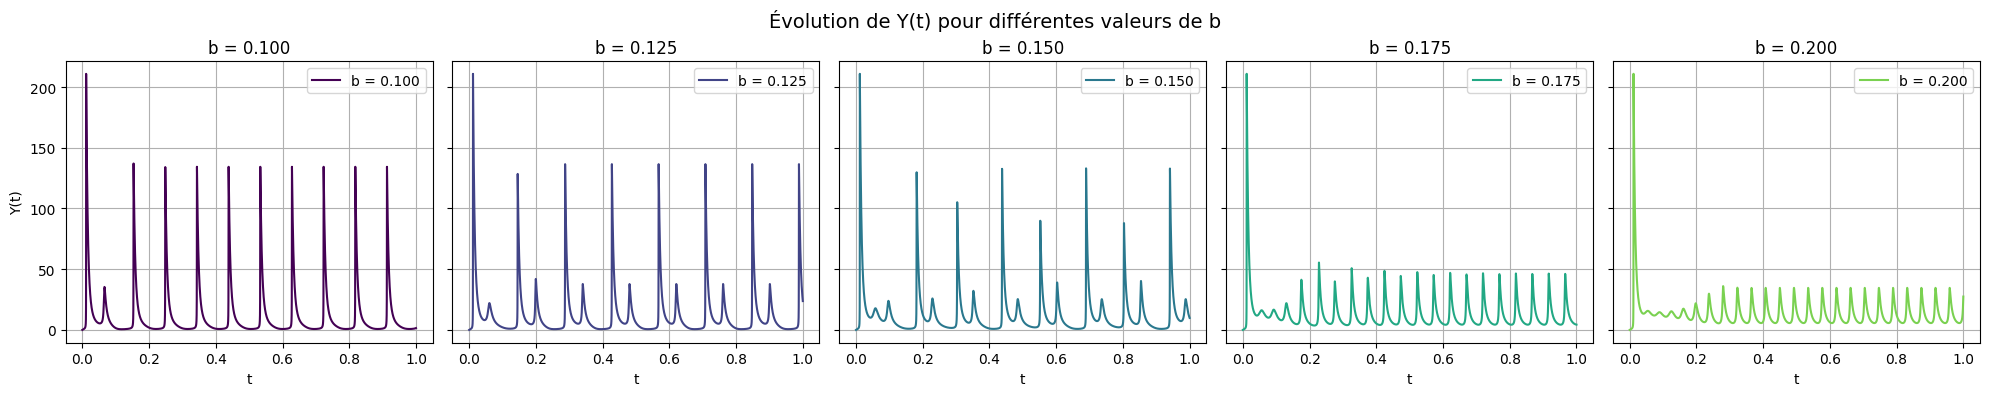
\includegraphics[width=\textwidth]{../code/resolution.png}
\caption{Comportement du système selon $b$}
\label{fig:oscillations}
\end{figure}

On observe que le système oscille, et que l'amplitude ainsi que la fréquence des pics de $Y(t)$ varient avec $b$ : plus $b$ augmente, plus les oscillations deviennent complexes.

\subsection{Analyse des périodes et bifurcations}

Une fonction \verb|periode_solution(b)| détecte les intervalles entre pics de $Y(t)$ à l'aide de \verb|find_peaks| (\texttt{scipy}). En regroupant les intervalles similaires, nous identifions la période du système.

En balayant différentes valeurs de $b$, aucune période 2 à 5 n'a été détectée, mais un comportement chaotique (avec de nombreuses périodes différentes) apparaît vers $b \approx 0.150$, avec des intervalles irréguliers tels que :
{-193.011, -107.702, ..., 105.823}

\subsection{Diagramme de bifurcation}

Le diagramme de bifurcation ci-dessous représente les valeurs de $Y(t)$ aux pics en fonction de $b$ :

\begin{figure}[H]
\centering
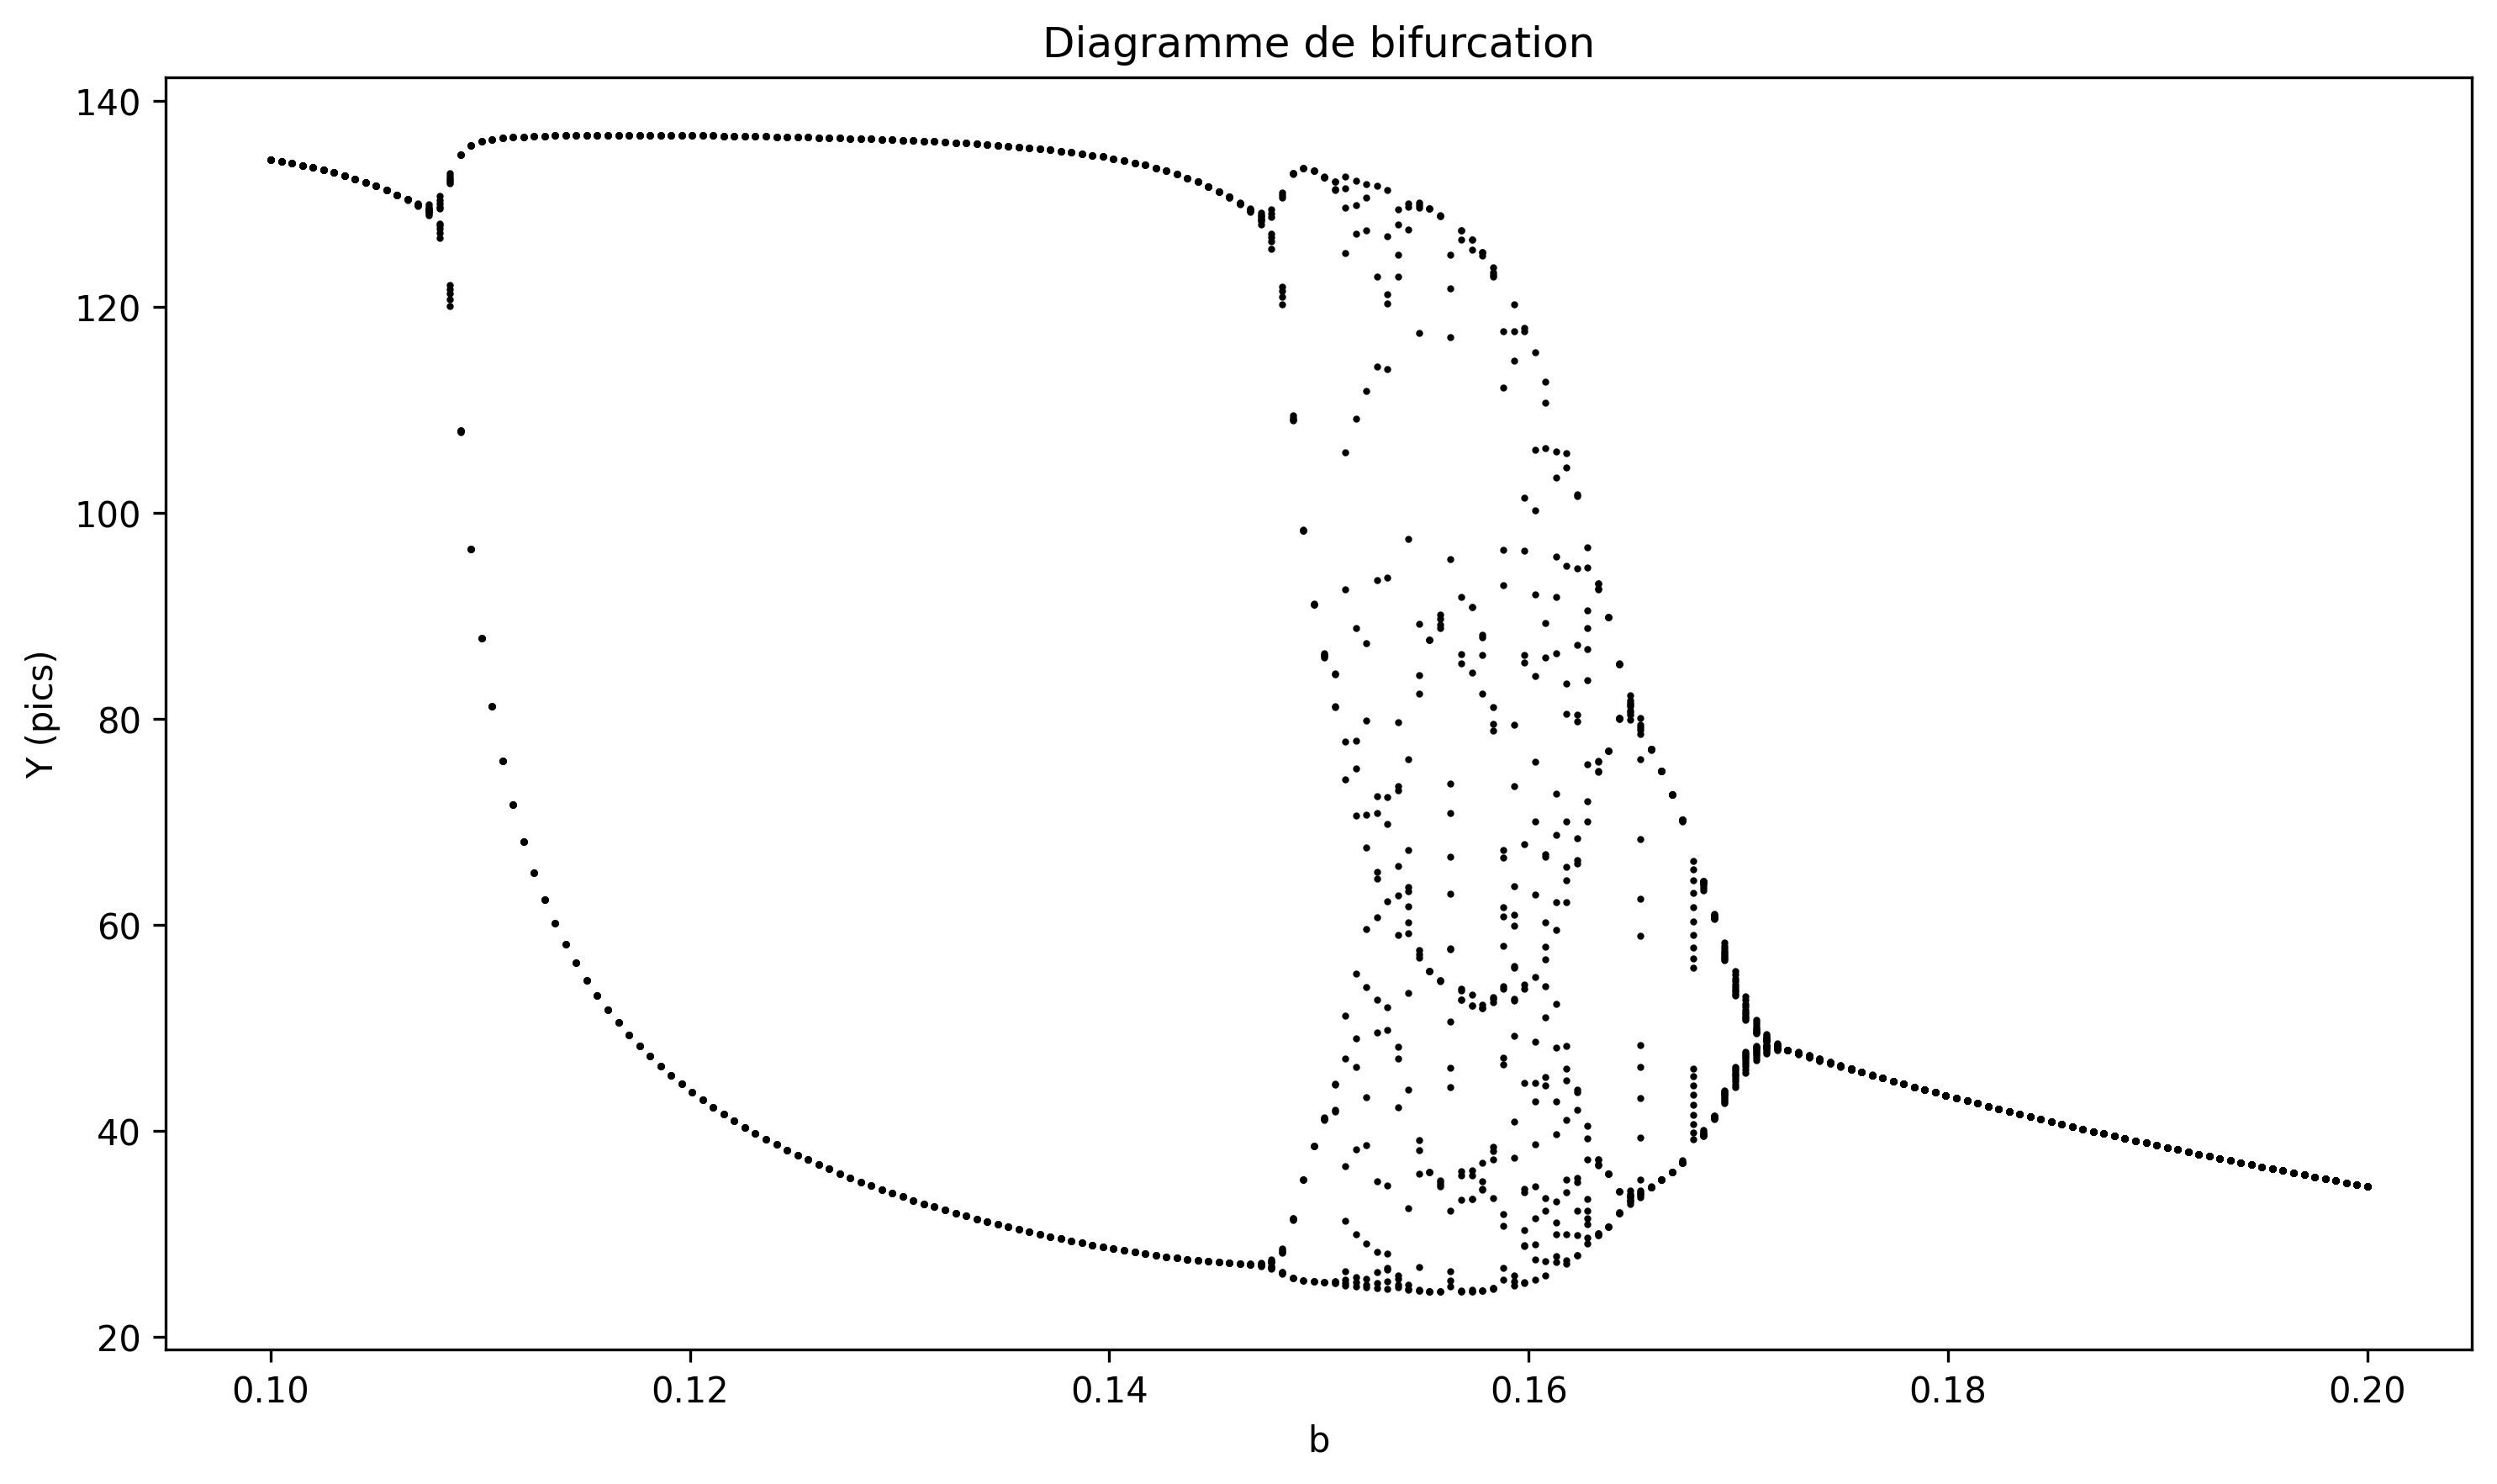
\includegraphics[width=0.85\textwidth]{../code/bifurcation.png}
\caption{Diagramme de bifurcation en fonction de $b$}
\label{fig:bifurcation}
\end{figure}

On y voit clairement la transition d'un comportement périodique à un régime chaotique, avec une multiplication des attracteurs.

\subsection{Chaoticité et lien avec la période 3}

Selon le théorème de Li et Yorke (\textit{Period three implies chaos} \citep{reaction}), l'existence d'une période 3 implique du chaos. Ce n'est pas observé ici, mais les irrégularités et la sensibilité au paramètre $b$ suggèrent fortement une dynamique chaotique.

\subsection{Difficultés numériques}

La simulation de systèmes chaotiques pose plusieurs défis :
\begin{itemize}
    \item Sensibilité aux conditions initiales
    \item Propagation exponentielle des erreurs
    \item Choix critique du pas de temps
    \item Distinction entre chaos réel et bruit numérique
\end{itemize}
    
Nous avons utilisé un pas de $h = 10^{-6}$ avec RK4 pour limiter ces effets, mais les imprécisions restent inévitables dans les zones sensibles.

\section{Étude dynamique du pendule à N maillons}

\subsection{Modélisation du pendule simple (un maillon)}

Nous commençons par l’étude du pendule simple, constitué d’un seul maillon de longueur \( l \), de masse \( m \), soumis à la gravité. Son mouvement est entièrement décrit par un angle \( \theta(t) \), mesuré entre la verticale et la tige. L'équation différentielle régissant son mouvement est :

\[
\frac{d^2\theta}{dt^2} + \frac{g}{l} \sin(\theta) = 0,
\]

où \( g \) est l’accélération due à la gravité. Pour de petites oscillations, on peut linéariser cette équation en approximant \( \sin(\theta) \approx \theta \), ce qui donne une fréquence propre \( f = \frac{1}{2\pi} \sqrt{\frac{g}{l}} \).

Nous avons implémenté une fonction qui, pour un angle initial \( \theta_0 \), calcule la période moyenne du pendule à l’aide de différents schémas d’intégration numérique. La fréquence associée est ensuite calculée en faisant l’inverse de cette période. La figure \ref{fig:simple_pendulum} illustre l’évolution de cette fréquence en fonction de \( \theta_0 \), mettant en évidence le fait que la fréquence devient quasi constante pour des petites amplitudes, en accord avec la théorie linéarisée.

\begin{figure}[H]
    \centering
    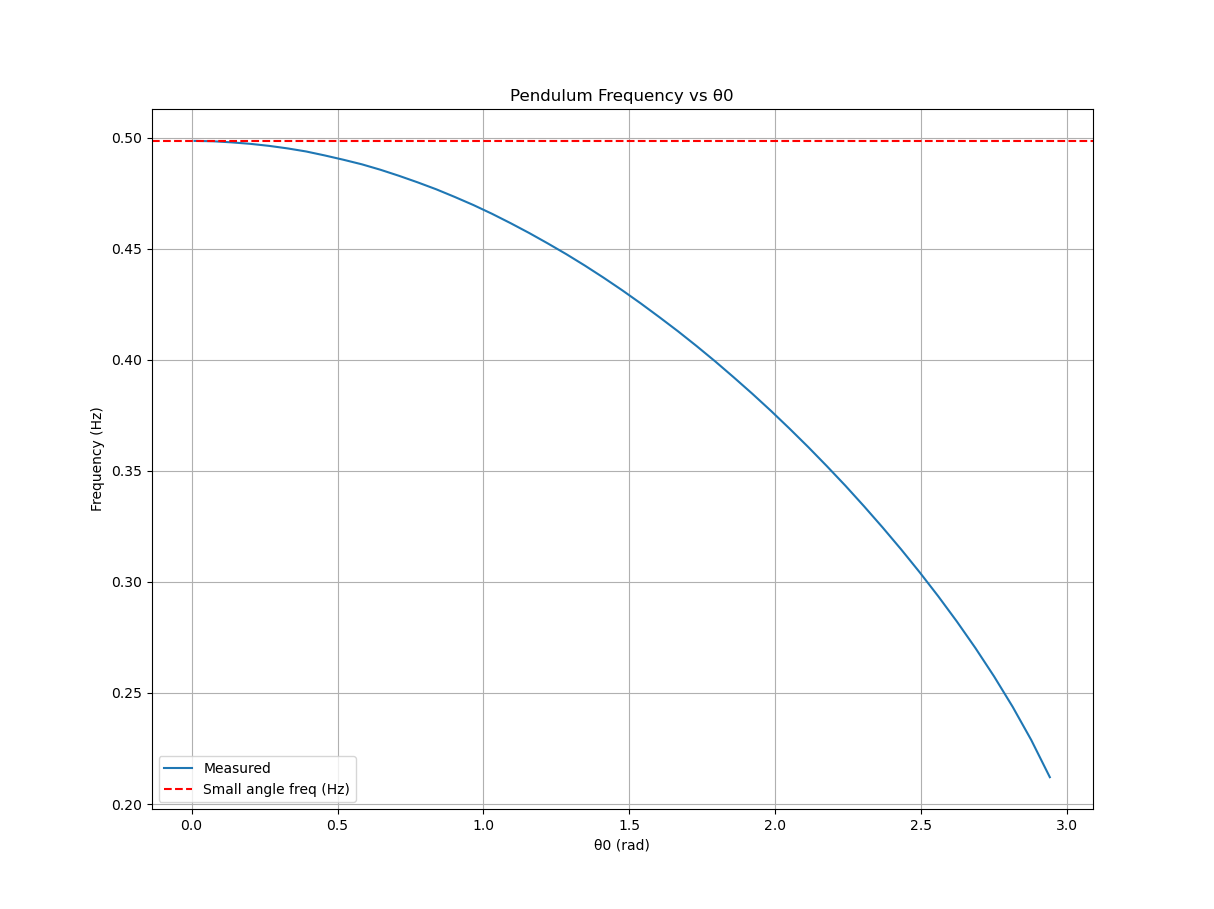
\includegraphics[width=0.5\linewidth]{img/Simple_pendulum_frequency.png}
    \caption{Fréquence d’oscillation du pendule simple en fonction de l’angle initial \( \theta_0 \). La fréquence tend vers \( \sqrt{g/l}/(2\pi) \) pour les petites oscillations.}
    \label{fig:simple_pendulum}
\end{figure}

\subsection{Modélisation du pendule double (deux maillons)}

Nous étudions ensuite le pendule double, système dynamique constitué de deux tiges de longueurs \( l_1 \) et \( l_2 \), de masses respectives \( m_1 \) et \( m_2 \), articulées en série. Ce système est modélisé par deux angles \( \theta_1(t) \) et \( \theta_2(t) \), correspondant aux positions des deux maillons. Les équations du mouvement sont obtenues par application des lois de la mécanique.

Ce système présente un comportement chaotique : de petites variations dans les conditions initiales peuvent conduire à des trajectoires radicalement différentes. Cette sensibilité est illustrée par la figure \ref{fig:double_pendulum}, où l’on observe la trajectoire de l’extrémité du second maillon pour des conditions initiales légèrement différentes.

\begin{figure}[H]
    \centering
    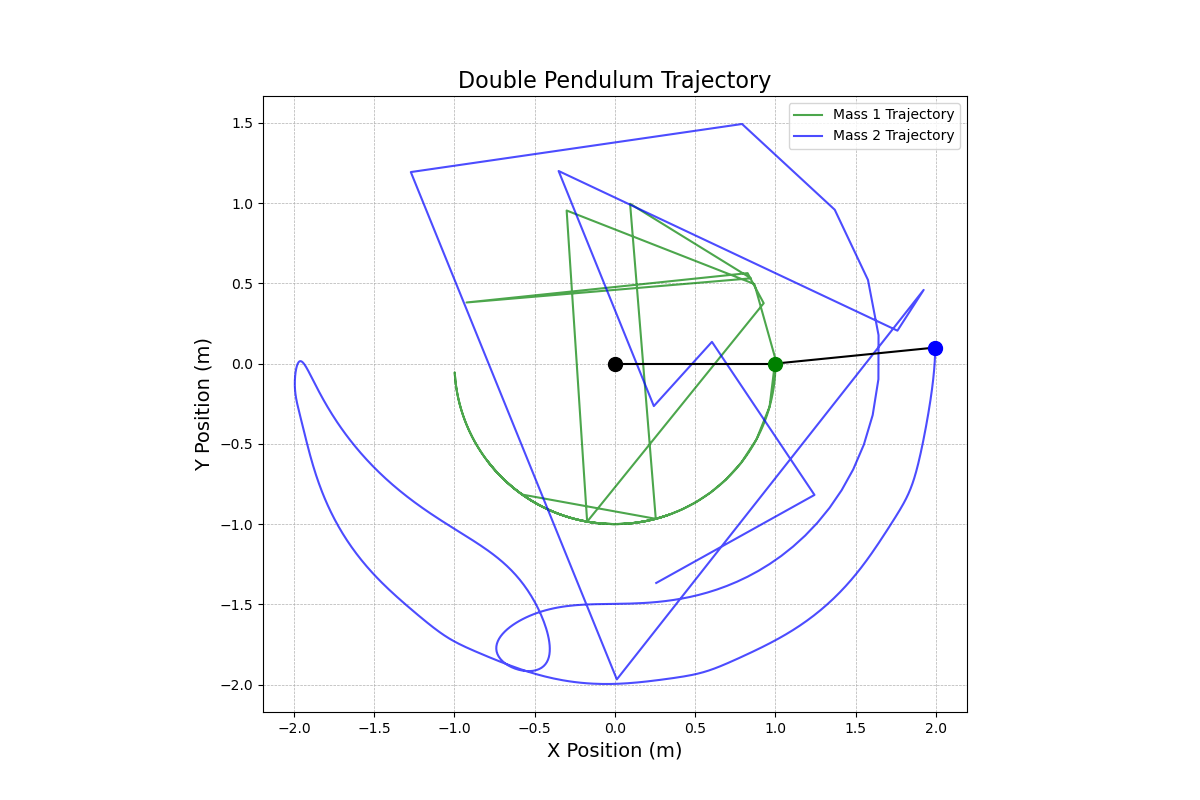
\includegraphics[width=0.6\linewidth]{img/Double_pendulum_motion.png}
    \caption{Trajectoires de l’extrémité du pendule double pour des conditions initiales proches. Les divergences soulignent le comportement chaotique du système.}
    \label{fig:double_pendulum}
\end{figure}

\subsection{Temps de premier retournement}

Pour quantifier le comportement chaotique, une méthode consiste à mesurer le \textit{temps de premier retournement}, c’est-à-dire le temps mis par le pendule pour effectuer un demi-tour complet à partir de sa position initiale. Nous avons conçu une fonction qui détecte ce moment en resolvant les equations du mouvement. En effectuant cette mesure pour un grand nombre de conditions initiales, nous avons pu générer une carte de couleurs représentant le temps de retournement, illustrée en figure \ref{fig:first_flip}.

\begin{figure}[H]
    \centering
    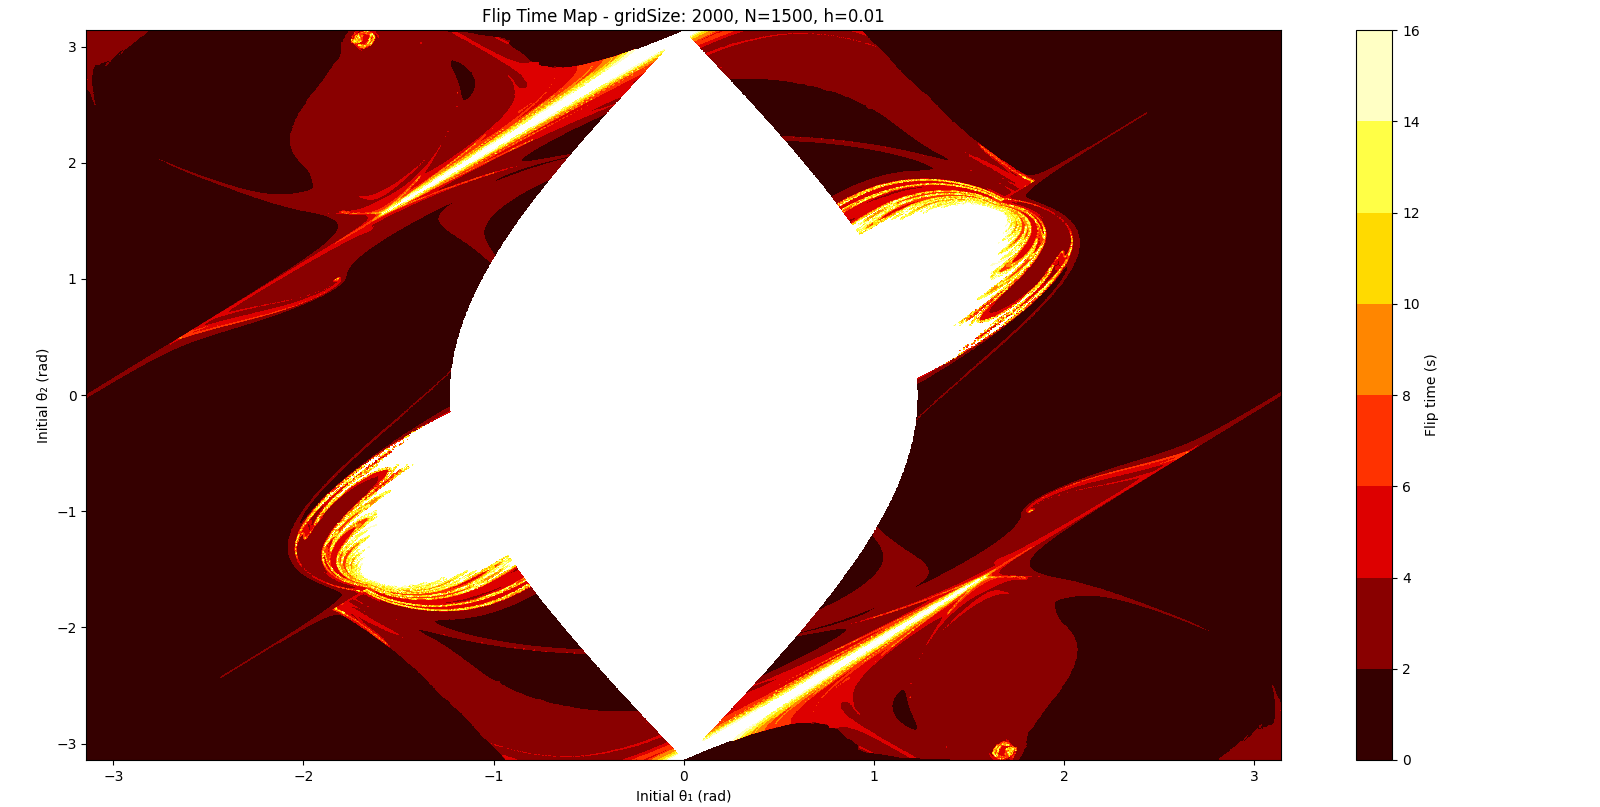
\includegraphics[width=0.75\linewidth]{img/First_flip_map.png}
    \caption{Carte du temps de premier retournement en fonction des conditions initiales \( \theta_1 \) et \( \theta_2 \). Les variations brutales de couleurs trahissent la complexité du système.}
    \label{fig:first_flip}
\end{figure}


\bibliographystyle{plainnat}

\begin{flushleft}
  \bibliography{references}
\end{flushleft}

\end{document}
